%-------------------------------------------------------------------
% bachelor thesis
% create by: Mario Preishuber
% create date: 2014, Jan 01.
%-------------------------------------------------------------------

\section{System Heap Analysis}  \label{sec:analysis_system}

In this section we present our analysis results of the system heap. For our analysis we only care about objects of type hidden, native, or synthetic. Objects of type hidden represent hidden classes. These objects are generated by Google's V8 and represent the properties of a object. GC roots has the type synthetic and objects of type native represent other objects, i.e., DOM roots. We analyze the same properties as described in Section \ref{sec:analysis_mutator} in the same way.

The result of the object type distribution of the system types show that about 99\% of these objects are of type hidden, this holds for all workloads. There are extreme few objects of the types synthetic and native. One reasons is that objects of type synthetic represent GC roots and it is plausible that there are not much such objects. Nevertheless, we care about them, because of completeness.

Figure \ref{fig:obj_sys_selfsize_dist} illustrates the size distribution of the system object types of all snapshots over all workloads. The size of native and synthetic objects is always zero in a heap snapshot. This is a special behavior and represents not the real size of these objects. Nevertheless, is Figure \ref{fig:obj_sys_selfsize_dist} interesting because is shows the size distribution of hidden classes. On the x-axis of the figure the size in byte and on the y-axis the relative amount of objects smaller than size x. We see that there are only few objects of type hidden with a size larger than 64 byte. It seems that the size of 64 byte is some kind of bound, because there is a hard back. 

\begin{figure}
	\centering
	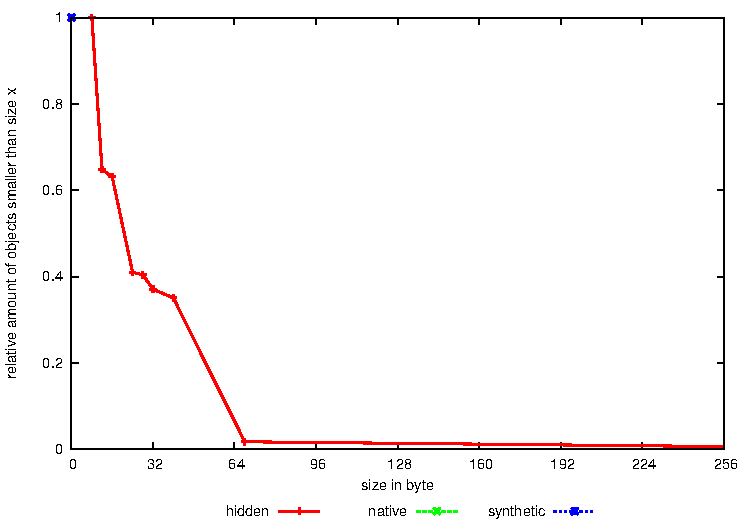
\includegraphics[width=0.5\textwidth]{obj_sys_selfsize_dist}
	\caption{Size distribution of real web applications.}
	\label{fig:obj_sys_selfsize_dist}
\end{figure}

In Figure \ref{fig:obj_sys_lieftiem_dist} we present the lifetime distribution over all snapshots of all workloads separated by the object type. The x-axis shows the object lifetime in allocated KB. We decided to use this metric to get rid of the lifetime in snapshots representation. The sample rate of the snapshot generation is 4KB of allocated memory and this leads to an minimum lifetime of 4KB. The lifetime of hidden classes shows a similar behavior than the lifetime of mutator objects of type user-defined object as explained in Section \ref{sec:analysis_mutator}, especially Figure \ref{fig:obj_lifetime_dist} on page \pageref{fig:obj_lifetime_dist} illustrates this behavior.

\begin{figure}
	\centering
	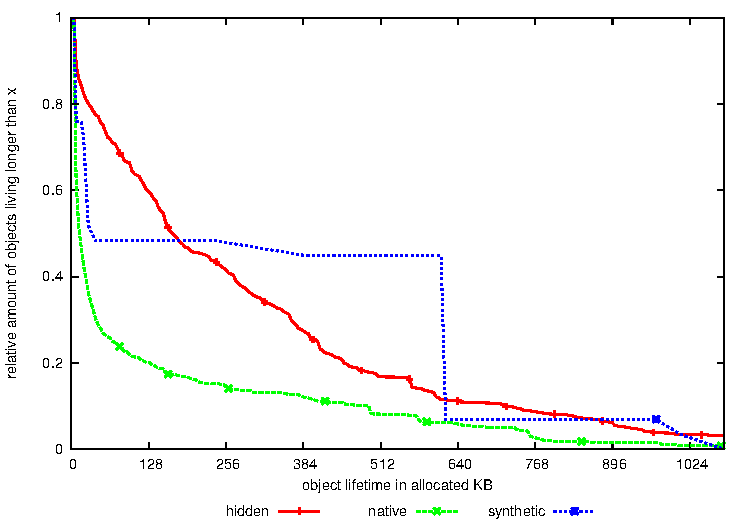
\includegraphics[width=0.5\textwidth]{obj_sys_lifetime_dist}
	\caption{Lifetime distribution of real web applications.}
	\label{fig:obj_sys_lieftiem_dist}
\end{figure}

The root distance of nodes in a graph is an interesting parameter of the graph characteristic. If we look at the root distance of system objects we face some special cases, because objects of type synthetic represent GC roots that are used to compute the root distance. It is possible that an object of type synthetic also has an root object. So the root distance of synthetic objects is always zero or one. Objects of type native show a similar behavior because these are also used to represent DOM roots. Nevertheless, the behavior of objects of type hidden provides interesting information. Figure \ref{fig:obj_sys_rootdist_dist} illustrates the root distance distribution of system objects. The x-axis of the figure shows the minimum root distance and the y-axis the relative amount of objects with a root distance smaller than x. We conclude that hidden classes have a small root distance and that there are only few objects with a higher root distance.

\begin{figure}
	\centering
	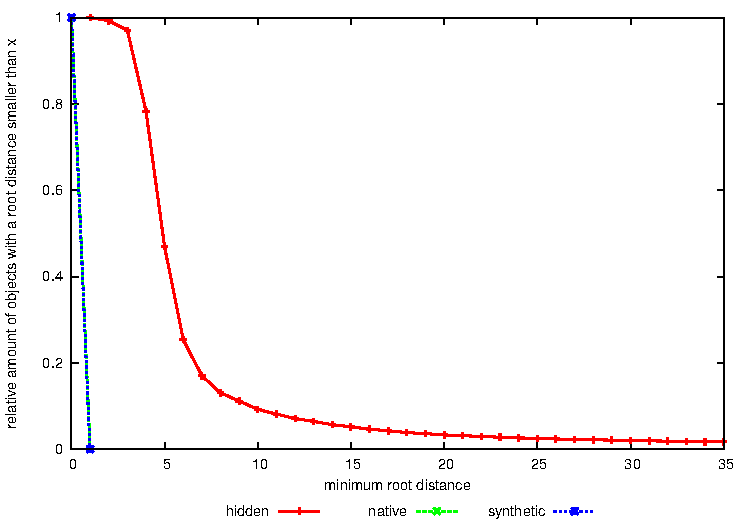
\includegraphics[width=0.5\textwidth]{obj_sys_rootdist_dist}
	\caption{Root distance distribution of real web applications.}
	\label{fig:obj_sys_rootdist_dist}
\end{figure}

The Figure \ref{fig:obj_sys_outdeg_dist} presents the distribution of outgoing
edges of a node, the so-called out-degree. This illustration shows the results
computed over all snapshots of all workloads. In this figure we see that
objects of type hidden have a out-degree of less than ten. If we have a look at
the native line, we recognize that this kind of objects have a significantly
higher out-degree than objects of type hidden. Especially objects of type
synthetic have a extreme high out-degree, because they represent the GC roots
and we conclude that the heap tree is very breadth.

\begin{figure}
	\centering
	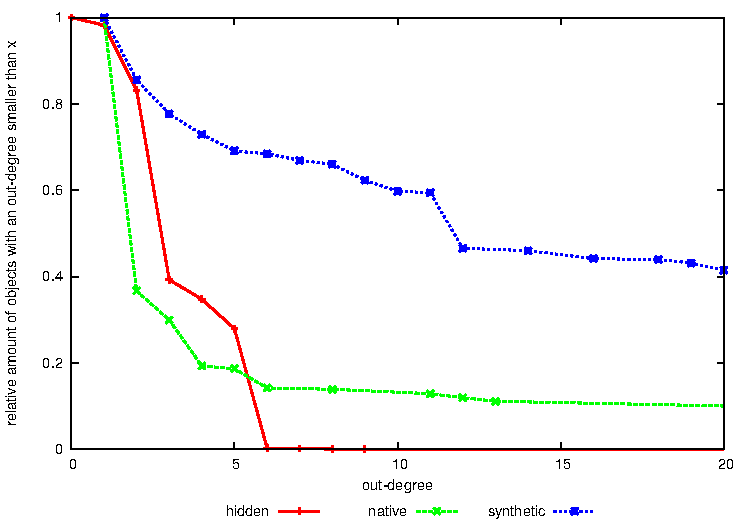
\includegraphics[width=0.5\textwidth]{obj_sys_outdeg_dist}
	\caption{Out-degree distribution of real web applications.}
	\label{fig:obj_sys_outdeg_dist}
\end{figure}

% \begin{figure}
% 	\centering
% 	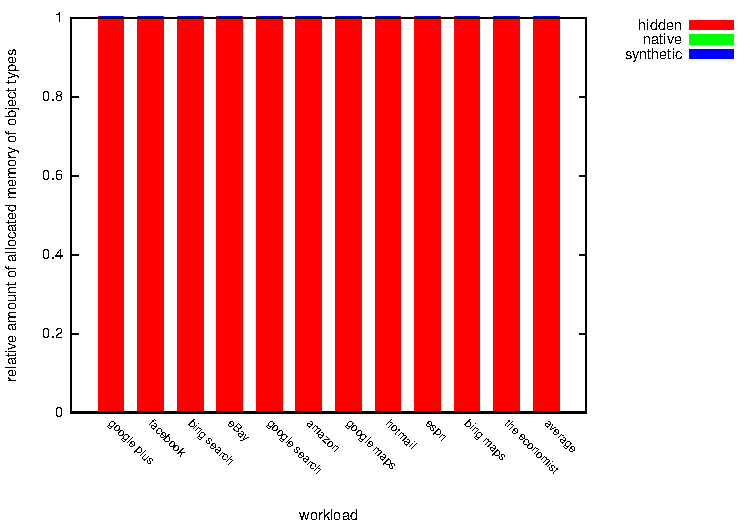
\includegraphics[width=0.5\textwidth]{obj_sys_byte_dist}
% 	\caption{Histogram of the object type distribution for all workloads.}
% 	\label{fig:obj_sys_byte_dist}
% \end{figure}
% 
% \begin{figure}
% 	\centering
% 	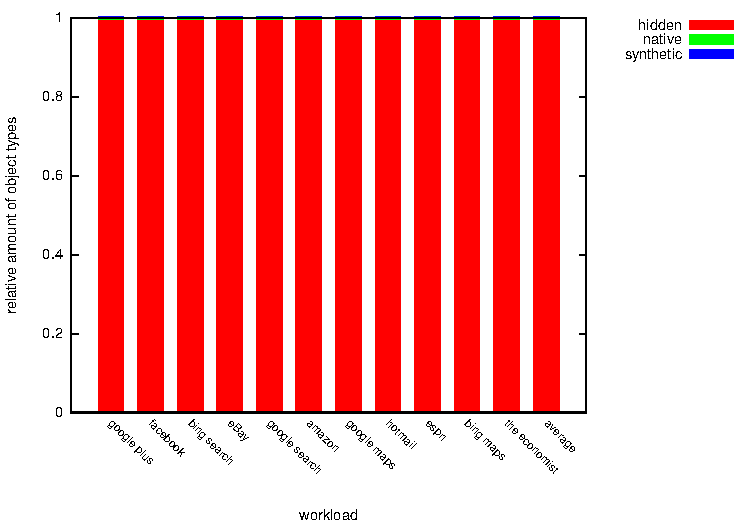
\includegraphics[width=0.5\textwidth]{obj_sys_alloc_dist}
% 	\caption{Histogram of the object type distribution for all workloads.}
% 	\label{fig:obj_sys_alloc_dist}
% \end{figure}
